\chapter{Evaluation}
\label{ch:evaluation}

The synchronized hybrid editor has been evaluated in three steps. We first made a qualitative evaluation in order to determine how the requirements were met and we discovered some gaps that were subsequently corrected. Then, we evaluated our work quantitatively by analyzing the time performance of the graphical functions and of the synchronization module. Finally, we made an user evaluation that helped us assess the usability and the practicality of our editor. 

\section {Meeting the Requirements}

While evaluating the functionalities of the editor with respect to the requirements formulated in \autoref{ch:requirements}, we discovered some mismatches and aspects that could still be improved.

Regarding \textbf{graphical editing}, the manipulation module for altering data in the network, offered by \textit{vis.js}, pretty much covered our needs. However, we realized that, although the parsing library accepts and recognizes automatically labels surrounded by quotes as literals, the user was not informed in any way about this functionality. We decided that an enhancement of the ``Add node'' form is needed. Therefore, we added a tooltip that clarifies the possibility of adding two different types of nodes: an URI entity or a string literal.

The \textbf{synchronization} module did not require many subsequent modifications either. One inconsistency that we observed is concerned with updating the code view after adding in the network a new node with a label that is not quoted and also not prefixed with any namespace. In this case, we first considered the label as the node's URI and it was displayed in the text view exactly as introduced by the user. This was correct only as long as there was no base prefix specified in the code. Later on, we added an extra check for a base prefix and, in case it was found, we prepended it to the specified label. Another observation came with regard to term highlighting. Initially, we made a plain string search by the label of the selected node, but we noticed that other entities can be matched too, although they are semantically different. This was the case of URIs that partially contained the searched string. We concluded that a match by meaning is needed and we implemented a pattern search in order to ensure that the highlights are performed exclusively for the selected entity.

The \textbf{visualization} was evaluated in multiple stages and we gradually added different improvements for enhancing the user interaction with the graphical representation of the RDF data. Among these, we mention:

\begin{itemize}
	\item coloring the literals differently: we considered a clear visual distinction was needed between URI entities and string literals.
	\item truncating the nodes' labels at 15 characters: since the labels determine the size of the nodes, we decided that a certain uniformity is required for a pleasant visualization of the graph.
	\item hiding defaults implicitly when the network is initially drawn: as pointed out in \autoref{subsec:visualization}, even in the case of small graphs, the visualization is noticeably clearer when nodes from the RDF, RDFS and OWL namespaces are not displayed; therefore, we decided that this feature should be implemented as a default.
	\item the possibility to hide the editing toolbar: we noticed that on smaller devices, the space occupied by the toolbar could negatively impact the network navigation, so we concluded that the user shall be able to temporarily suppress it.
	\item increasing repulsion as the size of a cluster grows: initially, the repulsion's value was static, but since the size of the node was calculated dynamically (it increases with the number of children), a certain discrepancy could appear in the graph display; therefore, for improving the visibility, we decided that computing the repulsion dynamically (with respect to the number of contained nodes) is also required.
	\item tooltips for hiding default nodes and freezing the network movements: additional explanations were considered useful for users which are not familiar with RDF data and methods for displaying it.
\end{itemize}


\section {Time Performance}

The web editor has been evaluated quantitatively by analyzing the time performance of the initial network load and of the two-way synchronization. The evaluation tests were run using the Google Chrome web browser (version 54), in an environment with an i5 CPU with two physical cores of 2.66 GHz each, 4 GB RAM and 64-bit operating system (Windows 8.1). 

In order to perform these measurements, we chose five files containing ontologies of different sizes, as follows:

\begin{itemize}
	\item O1 - 27 triples
	\item O2 - 77 triples
	\item O3 - 178 triples
	\item O4 - 513 triples
	\item O5 - 1573 triples
\end{itemize}

While evaluating the time needed for the initial load of a network (that is, when a file is loaded in the TurtleEditor), we noticed that, in the case of larger ontologies (O3, O4 and O5), approximately 70\% of the time is consumed by the physics module, which uses a multiple-step method to calculate the forces exerted between nodes. As a result, we considered three scenarios:

\begin{enumerate}
	\item physics module is enabled with default values.
	\item physics module is enabled with custom values, which are intended to improve the time performance, as explained in \autoref{subsec:visualization}; also clustering is applied for ontologies larger than 500 triples. 
	\item physics module is disabled.
\end{enumerate}

\begin{figure}[htb]
	\centering
  	\centerline{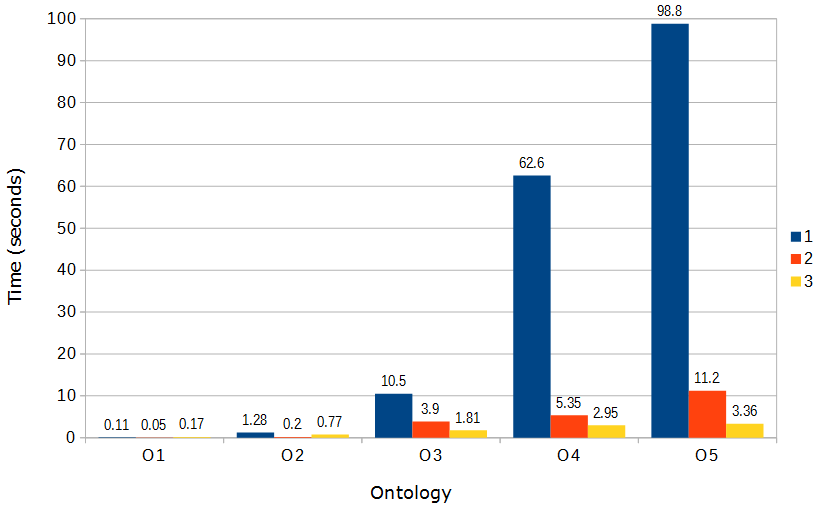
\includegraphics[width = \textwidth]{img/initial_load.png}}
	\caption{The time (in seconds) taken for the initial network load in each of the three scenarios, grouped by ontology.}
	\label{img:initial_load}
\end{figure}

The results of our measurements, for each of the three scenarios, are presented in \autoref{img:initial_load}. In the third case, when the physics are completely absent, most of the time is consumed by operations like parsing the Turtle code, manipulating the resulting array of triples and initializing the network with these data. Although it yields by far the best results with respect to time performance, we chose the second scenario for our final implementation. The reason for this decision is that, when the algorithms within the physics module are not applied, the resulting graph is almost unreadable as many nodes are overlapping each other due to the lack of repulsion forces. Moreover, after the network load, the physics can be disabled in order to decrease the memory consumption of the web browser. At the same time, the layout that was previously calculated when the module was active, is preserved.

In order to evaluate the time needed for updating the graphical view as a result of a textual modification, we considered two situations regarding the data structure that is used for performing the symmetrical difference between the old and the new triples. As discussed in \autoref{subsec:synchronization}, this operation is the most expensive one when it comes to propagating changes towards the visual side. The two structures are: plain Javascript arrays and N3 Stores (offered by the \textit{N3.js} library). The code change performed for each situation was erasing a letter from an entity's URI. The results are shown in \autoref{img:arrayVSstore}. As we can observe, the time does not vary too much in the case of the first four ontologies. Only for the largest ontology there is a considerable difference (almost one second), which is the reason why we chose to proceed with N3 Stores in our implementation.

The visual to text synchronization is a fast operation for all of the five ontologies. We measured the time taken when the label of a node is edited in the graphical view. The resulting time did not vary significantly among the cases, the difference between O1 and O5 being of only 200 milliseconds. \autoref{img:text_sync} shows how this time is distributed among the five ontologies.

\begin{figure}[]
	\centering
  	\centerline{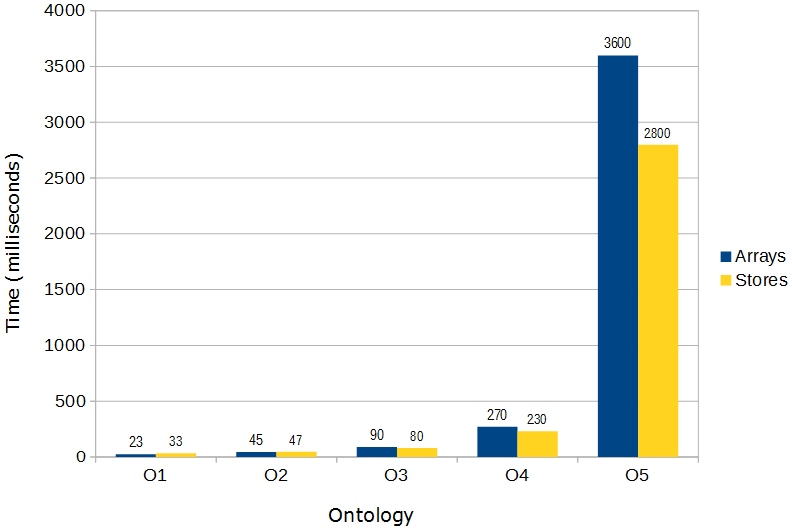
\includegraphics[width = \textwidth]{img/arrayVSstore.png}}
	\caption{The time (in milliseconds) needed to perform the text to visual synchronization with two different data structures for the model.}
	\label{img:arrayVSstore}
\end{figure}

\begin{figure}[]	
  	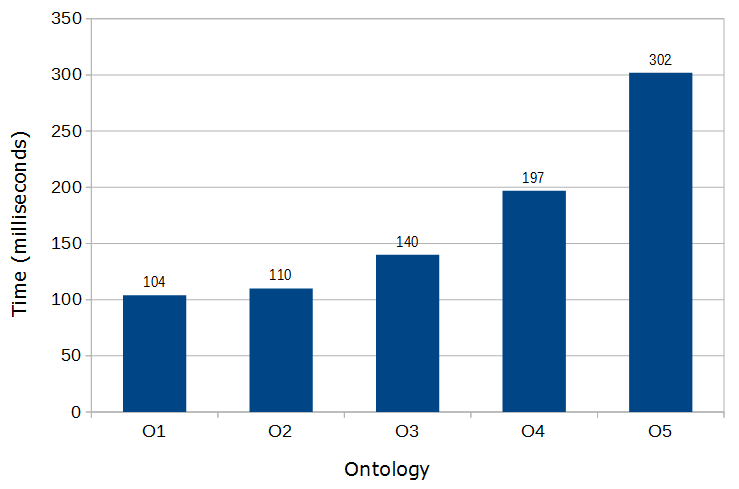
\includegraphics[width = 0.9\textwidth]{img/text_sync.png}
	\caption{The time performance (in milliseconds) of the visual to text synchronization, depending on the ontology size.}
	\label{img:text_sync}
\end{figure}


\section {User Evaluation}

In order to objectively evaluate the usability and practicality of our editor, we conducted a user study where the participants had to perform several tasks and then respond to a few questions that would assess their interaction with the application.

The experiment was done sequentially, meaning that the activity of each participant was observed and assisted individually, in order to better identify which functionalities may raise usability problems. At the same time, we were able to give hints when the user got stuck on a certain task and, hence, we made sure that the entire test is approached. We noticed that the users were generally identifying the same problems so we decided to end the experiment after the sixth participant, as the gathered data was already sufficient.

Previous experience and technical knowledge play a significant role in the ability to perform this exercise. Therefore, we selected exclusively subjects having a degree in computer science. On top of that, we made a survey with regard to their age and expertise in the semantic web field, placing emphasis on the area of ontology design. We asked each participant to estimate a time period since they got familiar with these domains and, in case they modeled any ontologies before, to specify what types of editors they used. All subjects that confirmed working with a graphical editor, indicated Protégé as their choice.  The results are presented in \autoref{tab:experience}.

\begin{table}[htb]
\centering
\begin{tabular}{|c|c|c|c|c|}
\hline
\textbf{\begin{tabular}[c]{@{}c@{}}Participant\\ identifier\end{tabular}} & \textbf{Age} & \textbf{\begin{tabular}[c]{@{}c@{}}Semantic\\ web\end{tabular}} & \textbf{\begin{tabular}[c]{@{}c@{}}Ontology\\ design\end{tabular}} & \textbf{\begin{tabular}[c]{@{}c@{}}Editors\\ type\end{tabular}} \\ \hline
P1                                                                        & 24           & 4 years                                                         & 2 years                                                            & \begin{tabular}[c]{@{}c@{}}graphical\\ and code\end{tabular}    \\ \hline
P2                                                                        & 34           & 1 year                                                          & 2 months                                                           & \begin{tabular}[c]{@{}c@{}}graphical\\ and code\end{tabular}    \\ \hline
P3                                                                        & 29           & 1 year                                                          & 5 months                                                           & only code                                                       \\ \hline
P4                                                                        & 29           & 4 years                                                         & 3 years                                                            & \begin{tabular}[c]{@{}c@{}}graphical\\ and code\end{tabular}    \\ \hline
P5                                                                        & 35           & 10 years                                                        & 9 years                                                            & \begin{tabular}[c]{@{}c@{}}graphical\\ and code\end{tabular}    \\ \hline
P6                                                                        & 29           & 6 months                                                        & -                                                                  & -                                                               \\ \hline
\end{tabular}
\caption{Background data about the user study participants.}
\label{tab:experience}
\end{table}

The evaluation test consisted of nine tasks which aimed to bring a set of modifications to an already existing ontology. They were structured as follows: first three tasks for familiarizing with the interface, tasks 4 - 8 for using the graphical editor functionalities and the last one to be performed with the code editor:

\begin{enumerate}
	\item Load \textit{Country.ttl}. Go to the graphical view and add another language label for \textit{mv:Country} (e.g. ``Pays''@fr).
	\item Uncheck ``Hide defaults'' in order to see the nodes from the RDF, RDFS and OWL vocabularies.
	\item Click ``Split view''.
	\item Define a new property by adding a node (e.g. ``Prop1'') and make it of type (rdf:type) \textit{rdf:Property}. Note that the \textit{rdf:Property} node already exists.
	\item Click on the new node to see it in the text.
	\item Make \textit{mv:Country} the property's domain (rdfs:domain) and \textit{rdfs:literal} its range (rdfs:range). Note that the \textit{rdfs:literal} node already exists.
	\item Add a description for the property.
	\item Modify the node's label (e.g. ``Prop2'').
	\item Remove the property.
\end{enumerate}

We noticed that the speed to which the participants performed these tasks is correlated to their level of experience, especially when previous ontology design is involved. On average, the time needed to solve the entire test amounted to approximately 15 minutes. \autoref{img:user_time} shows how this time is distributed among the participants.

\begin{figure}[htb]
	\centering
  	\centerline{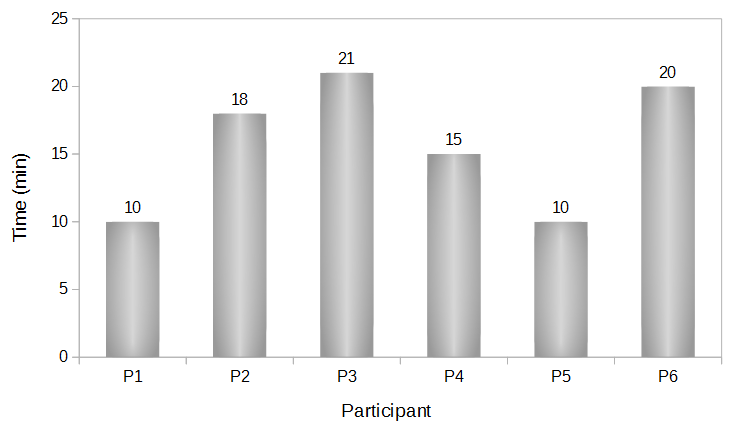
\includegraphics[width = \textwidth]{img/user_time.png}}
	\caption{Time (in minutes) taken by each participant for solving the test.}
	\label{img:user_time}
\end{figure}

While observing the participants' activity, we noticed that most of them encountered two problems. First was the edge drawing - except P1, they all expected that the edge will appear if the nodes that need to be linked are clicked consecutively. The actual method (clicking the first node and holding the click while dragging the edge to the other node) appeared unexpected, even though there was an explanation in the manipulation toolbar, as it was shown in \autoref{img:toolbar}(f). The second problem was differentiating between an URI node and a string literal - except P6, the participants omitted the tooltip explaining that, in order to add a literal, its label has to be enclosed in quotes. Besides these two problems, for participants P1, P3 and P5, it was not clear that, when drawing an edge, its direction will imply which node is the subject and which is the object. Also,  P2, P3 and P5 found it cumbersome to locate the already existing nodes in the graph in order to link them with the newly added ones. Finally, P6 had difficulties in figuring out how to edit the graphical view - the ``Edit'' button needed to be clicked in order to display the manipulation toolbar, as show in \autoref{img:toolbar} (a) and (b). To draw a conclusion, we noticed that previous experience with other graphical tools might also have a negative effect, as it is expected that there are certain standards and every editor would work in the same way, which currently is not the case. Nevertheless, problems that were widely encountered among the participants indicate that some functionalities need to be changed in order to provide an usable tool which can become largely used within the ontology design communities.

After performing the tasks, the participants were asked to answer two questions. The first one consisted of three statements where the user had to indicate how much they agree with and the second one was an open-answer question:

\begin{enumerate}
	\item How much do you agree with each of the following statements?
	\begin{enumerate}
		\item The graph visualization represents the information in an understandable way.
		\item The graphical editor is intuitive to use.
		\item The synchronization helps with understanding the code representation in Turtle.
	\end{enumerate}
	\item Do you have any suggestions? (e.g. features you would improve / add)
\end{enumerate}

The level to which the participant agrees to the statements in the first question could be expressed by choosing one of the following affirmations:

\begin{itemize}
	\item Strongly agree (4)
	\item Somewhat agree (3)
	\item Neutral (2)
	\item Somewhat disagree (1)
	\item Strongly disagree (0)
\end{itemize}

In parentheses, there is the score we assigned to each affirmation in order to easily assess the participants' ratings by visualizing them in a chart and, finally, by calculating an average. Statements (a) and (c) obtained an overall score of 92\%, while (b) got only 70\%. The study results can be viewed in \autoref{img:scores}.

\begin{figure}[htb]
	\centering
  	\centerline{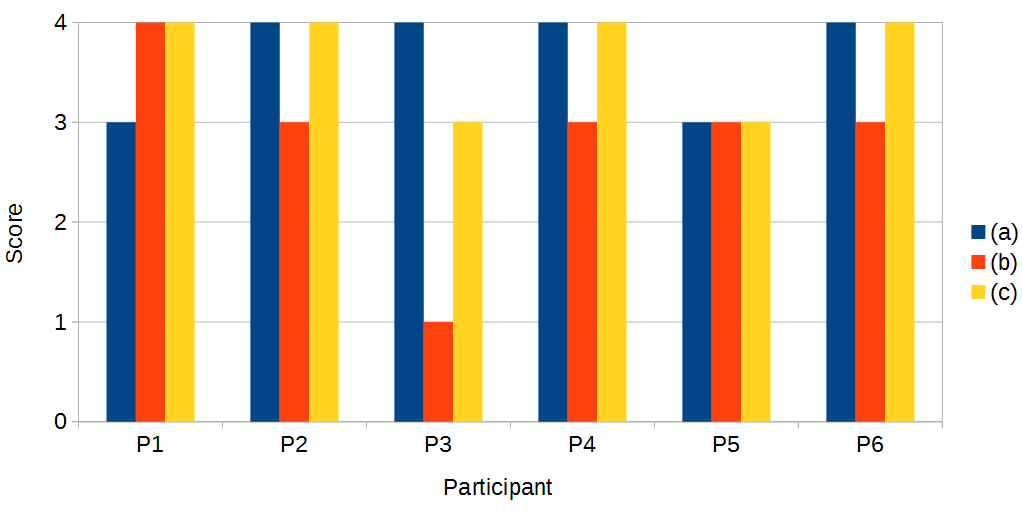
\includegraphics[width = \textwidth]{img/scores.png}}
	\caption{The scores obtained by each of the three statements in the first question, grouped by participant.}
	\label{img:scores}
\end{figure}

The answers to the second question helped us gather a set of suggestions for improvements and further development of the editor. The list below presents the recommendations made by the participants in the study:

\begin{itemize}
	\item P3, P5 and P6 - another way for drawing the edges. P3 suggested that edges could be drawn by clicking the two nodes consecutively. P5 and P6 preferred having a button available on the node's border, which will trigger edge drawing on click.
	\item P2 and P3 - another method to differentiate adding an URI node from a string literal. For example, not needing to include the label's text in quotes, rather having a dropdown menu or a radio button for choosing the type of the node.
	\item P4 and P5 - improvement for node locating in the graphical view. Similarly to the way text is highlighted when a node is clicked, the nodes or the edges also need to be focused depending on the position of the cursor in the text. Alternatively, a search functionality can be implemented for the graphical view, in order to be able to locate nodes or edges by their label.
	\item P1 and P5 - the options available in tabbed view (``Clustering'', ``Hide defaults'' and ``Freeze'') should also appear in split view.
	\item P1, P2,  P4 and P5 - auto-completion when typing the label of a node or edge in the graphical view.
	\item P1 and P4 - improvement for prefix handling as currently it is not possible to add nodes in the graph with prefixes that were not defined in the code.
	\item P1 - semantic check in both editors for preventing the creation of semantically incorrect triples.
	\item P1 - filters for different types of nodes in the graph (e.g. hiding all literals).
	\item P1 - support for typed literals as currently only string literals are differentiated from other nodes.
	\item P4 - disabling the graphical editing when there are errors in the code.
	\item P5 - having the ability to copy and paste graph elements.
	\item P5 - direct editing in the graph. When a node is clicked, editing its label should be enabled directly. In this way, there will be no need to click an edit button in order to modify the label in a form.
\end{itemize}

These suggestions will be part of the future work for further enhancing the hybrid editor.








